\documentclass[11pt]{article}

\usepackage[margin=1in]{geometry}
\usepackage[T1]{fontenc}
\usepackage{lmodern}
\usepackage{amsmath,amssymb,amsthm}
\usepackage{array}
\usepackage{enumitem}
\usepackage{float}
\usepackage{microtype}
\usepackage{tikz}
\usepackage{url}

\setlength{\parskip}{0.55em}
\setlength{\parindent}{1em}

\newtheorem{theorem}{Theorem}
\newtheorem{lemma}[theorem]{Lemma}
\newtheorem{proposition}[theorem]{Proposition}
\newtheorem{corollary}[theorem]{Corollary}
\newtheorem{observation}[theorem]{Observation}
\newtheorem{conjecture}[theorem]{Conjecture}
\theoremstyle{definition}
\newtheorem{definition}{Definition}
\newtheorem{example}[theorem]{Example}
\theoremstyle{remark}
\newtheorem{remark}[theorem]{Remark}
\newtheorem{problem}[theorem]{Problem}
\newcommand{\cF}{{\mathcal{F}}}
\newcommand{\ds}{\mathrm{ds}}
\newcommand{\dsi}{\mathrm{dsi}}
\newcommand{\ids}{\mathrm{ids}}
\newcommand{\diam}{\operatorname{diam}}
\newcommand{\dec}{\operatorname{dec}}
\newcommand{\forest}{\operatorname{forest}}
\newcommand{\bipnum}{\operatorname{bipartite}}
\newcommand{\bipcov}{\operatorname{bipartite\mbox{-}cover}}
\newcommand{\tw}{\operatorname{tw}}
\newcommand{\Core}{\operatorname{Core}_{\gamma}}
\newcommand{\iso}{\iota}
\newcommand{\pr}{\mathrm{pr}}
\newcommand{\ogamma}{\widetilde{\gamma}_{c}}
\newcommand{\avgdist}{\overline{d}}
\newcommand{\barG}{\overline{G}}
\newcommand{\barK}{\overline{K}}
\DeclareRobustCommand{\TheoConjecture}{\texttt{Theo-Conjecture}}
\DeclareRobustCommand{\AddDefinition}{\emph{Add Definition}}
\DeclareRobustCommand{\CoPilot}{\emph{Co-Pilot}}
\newcommand{\ArtifactRepo}{\url{https://github.com/RandyRDavila/dsi-domination-artifacts}}
\title{Dual-Server Independent Domination in Graphs}
\author{%
\begin{tabular}{>{\centering\arraybackslash}p{0.94\textwidth}}
Mustapha Chellali\({}^{1}\), Randy R. Davila\({}^{2,3,*}\), Teresa W. Haynes\({}^{4,5}\),\\
Stephen T. Hedetniemi\({}^{6}\), and Ryan Pepper\({}^{7}\)\\[0.75em]
\small \({}^{1}\)LAMDA-RO Laboratory, Department of Mathematics, University of Blida, B.P. 270, Blida, Algeria\\
\small \({}^{2}\)First Principles, 100 University Ave, Toronto, ON M5J 1V6, Canada\\
\small \({}^{3}\)Department of Computational Applied Mathematics \& Operations Research, Rice University, 6100 Main Street, Houston, TX 77005, USA\\
\small \({}^{4}\)Department of Mathematics and Statistics, East Tennessee State University, Johnson City, TN 37614, USA\\
\small \({}^{5}\)Department of Mathematics and Applied Mathematics, University of Johannesburg, Auckland Park, 2006, South Africa\\
\small \({}^{6}\)Emeritus College, Clemson University, Clemson, SC 29634, USA\\
\small \({}^{7}\)Department of Mathematics and Statistics, University of Houston--Downtown, Houston, TX 77002, USA\\[0.35em]
\small \({}^{*}\)Corresponding author: \texttt{randy@firstprinciples.org}
\end{tabular}}
\date{\today}

\begin{document}

\maketitle

\begin{abstract}
For a graph \(G=(V,E)\), a set \(S\subseteq V(G)\) is a \emph{dual-server dominating set} if
\(S\) can be partitioned into two subsets \(R\) and \(B\) such that every
vertex in \(V(G)\setminus S\) is adjacent to at least one vertex in \(R\) and at
least one vertex in \(B\). In this paper, we introduce and study two
independent versions of \emph{dual-server domination}. Specifically, if
\(S\) itself is independent, then \(S\) is an \emph{independent dual-server dominating set}; while if \(R\) and \(B\)
are independent sets, with no additional independence requirement on \(S\),
then \(S\) is a \emph{dual-server independent dominating set}. The latter notion is
the primary focus of the paper.  We prove that dual-server independent domination is well-defined for every nontrivial graph, establish basic comparison bounds, determine exact values for several
standard graph families, show that the parameter agrees with both
\emph{dual-server domination} and \emph{2-domination} on trees, and derive
sharp bounds in terms of \emph{order}, \emph{isolation number}, and
\emph{diameter}, including a characterization of equality for the isolation
bound. We also give a path-covering and matching upper bound for
dual-server domination, and hence, for DSI-domination on trees. Finally, we
show that, although the associated decision problem is NP-complete even for
chordal bipartite graphs, the parameter admits a compact binary integer programming
formulation and is polynomial-time solvable on graph classes of bounded
\emph{treewidth}. The work also records several roles played by the
AI-assisted system \TheoConjecture: its \AddDefinition{} tool led to the
binary integer programming formulation, its conjecture searches suggested
several of the bounds proved here, and its surviving conjectures, after
human and \CoPilot{} counterexample attempts, form the concluding
open-problems section.
\end{abstract}

\textbf{Keywords:} Domination; independent domination; dual-server domination;
2-domination; isolation number; path cover; matching number; diameter;
treewidth; NP-completeness.

\textbf{AMS subject classification:} 05C69 (2020).

\section{Introduction}

Domination in graphs has been extensively studied for more than fifty years,
with numerous variations developed to model different structural and applied
constraints. For a comprehensive treatment of domination in graphs, we refer
the reader to the books \cite{hhh1,hhh2,hhh3}. A set \(S\subseteq V(G)\) is a
\emph{dominating set} of a graph \(G\) if every vertex in \(V(G)\setminus S\) has a
neighbor in \(S\), and the minimum cardinality of such a set is the
\emph{domination number} \(\gamma(G)\).  A dominating set $S$ is an \emph{independent dominating set} of $G$ if $S$ is an independent set in $G$, and the minimum cardinality of such a set is the
\emph{independent domination number} \(i(G)\). Many variants of domination strengthen
this requirement by asking that vertices outside the dominating set receive
several forms of coverage, or by imposing internal structure on the dominating
set itself. The \emph{independent domination number}, the
\emph{2-domination number}, and related multiple-domination parameters are examples of
this general pattern.

Dual-server domination was introduced recently in~\cite{chh} as a two-service version of this
domination. A set \(S\subseteq V(G)\) is a dual-server dominating set if \(S\)
admits a partition \(S=R\cup B\) such that every vertex in \(V(G)\setminus S\)
has a neighbor in \(R\) and a neighbor in \(B\). Thus, vertices outside \(S\)
are served by both classes, which may be interpreted as two distinct types of
service. The partition is part of the structure: the same set \(S\) may admit
more than one dual-server partition, and the choice of partition may affect
additional restrictions placed on the two classes.

In this paper, we study independent restrictions on dual-server domination. There
are two natural possibilities. The more restrictive one requires \(S\) itself
to be independent, giving the direct analogue of independent domination. The
second requires only the two classes \(R\) and \(B\) to be independent,
allowing edges between the two classes but forbidding edges within either
class. We call these notions \emph{independent dual-server domination} and
\emph{dual-server independent domination}, respectively, and abbreviate them
as IDS-domination and DSI-domination. Accordingly, feasible sets for these two
notions will be called IDS-dominating sets and DSI-dominating sets. The
latter notion is the principal object of study here. It retains the
two-service interpretation of dual-server domination while imposing independence on each service class, and, unlike the
former, it exists for every nontrivial graph.



Although our focus is graph-theoretic, the two-color viewpoint also suggests
a modeling interpretation. In ensemble learning, diversity among predictors
is a central design theme \cite{Brown05,Dietterich00,Kuncheva04}, and
negative correlation learning explicitly penalizes correlated behavior
\cite{LiuYao99}. If vertices represent learners or data sources and
adjacency records a strong dependence relation, then a DSI-dominating set
selects two internally diverse representative panels that jointly cover the
remaining vertices. A similar two-panel interpretation may also be relevant
to multi-agent AI systems, where autonomous agents interact, cooperate, and
may require oversight or debate mechanisms
\cite{DafoeEtAl20,
IrvingChristianoAmodei18,ShohamLeytonBrown08,Wooldridge09}. Appendix~\ref{app:ensemble-experiment} records
two baseline computational illustrations of this interpretation; these are
included only as  motivation and are not part of the main
mathematical development of the paper.

\TheoConjecture{} is an AI-assisted automated conjecturing system implemented
within First Principles and developed in the lineage of TxGraffiti and
Graffiti3 \cite{DavilaTxGraffiti,DavilaGraffiti3}. At a high level, the
system maintains databases of mathematical objects and computable
invariants, searches those data for candidate relationships, tests proposed
statements against available examples, and exports selected conjectures for
human study. \TheoConjecture{} played three complementary roles in the
development of this work. First, its \AddDefinition{} tool was used
to introduce \(\gamma_{\dsi}\) as a new graph invariant in the First
Principles workspace database. In that workflow, a researcher supplies a
mathematical description of an invariant, the system drafts an executable
computation, and the draft is checked on small examples before being used in
larger searches. For \(\gamma_{\dsi}\), this process led to an exact binary
integer programming model. We include the mathematical form of that model in
Section~\ref{sec:computation}, both to make the computational experiments
reproducible and to make explicit how the two-color definition was encoded.

Second, after \(\gamma_{\dsi}\) was available as a computable invariant,
\TheoConjecture{} was used to search for candidate inequalities involving
standard graph parameters and structural graph classes. In particular, the
isolation lower bound in Theorem~\ref{thm:isolation}, the diameter lower
bound in Theorem~\ref{thm:diameter}, and the decycling-number specialization
in Proposition~\ref{prop:ids-forest} arose from this process.

Third, the open-problems section presents a curated list of remaining
conjectures generated by \TheoConjecture{} that survived both human
counterexample searches and counterexample attempts through the \CoPilot{}
chat interface. In this sense, the automated system served as a source of
definitions, computations, examples, comparisons, and problems, whereas the
statements, proofs, refinements, and interpretations that follow are the
mathematical contributions of the authors.




The paper is organized as follows. We prove the existence of dual-server independent domination 
for every nontrivial graph and establish comparison chains with other domination parameters. We determine values of dual-server domination parameters for several graph families and show that
on every nontrivial tree, DSI-domination agrees with both dual-server
domination and 2-domination. We then prove sharp bounds involving order,
isolation number, and diameter, determine a path-covering and matching bound
that is especially useful on trees, and give hereditary induced-subgraph
bounds involving forest and bipartite numbers.   Additionally, we give a compact
binary integer programming formulation, prove NP-completeness even for
chordal bipartite graphs, and derive a tractability result for bounded-treewidth instances.  We conclude with an 
open-problems section featuring selected conjectures  generated using \TheoConjecture{}.


All graphs in this paper are finite and simple. Let \(G=(V,E)\) be a graph
with vertex set \(V=V(G)\), edge set \(E=E(G)\), and \emph{order}
\(n=n(G)=|V(G)|\).  Let $\barG$ denote the \emph{complement} of $G$.
For a set \(S\subseteq V(G)\), we denote the subgraph induced by \(S\) by
\(G[S]\). For an integer \(k\ge 1\), we use the standard notation
\(i\in [k]\) to mean that \(i\) is an integer and \(1\le i\le k\).
The \emph{open neighborhood} of a vertex $v$ in $G$ is $N(v) = \{u \in V(G) \, \colon \, uv \in E\}$ and the \emph{closed neighborhood of $v$} is $N[v] = \{v\} \cup N(v)$.  The \emph{degree} of a vertex \(v\),  denoted by
\(\deg(v)\), is the cardinality of its open neighborhood.
The \emph{open neighborhood of a set} $S \subseteq V(G)$ is $N(S) = \bigcup_{v \in S}N(v)$, while the \emph{closed neighborhood of a set} $S\subseteq V(G)$ is the set $N[S] = \bigcup_{v \in S} N[v]$.  The \emph{minimum degree} and \emph{maximum degree} of \(G\) are
\(\delta(G)\) and \(\Delta(G)\), respectively. A vertex of degree one is a leaf, and its
unique neighbor is a support vertex.   The maximum cardinality of an independent set of $G$ is the \emph{independence number} \(\alpha(G)\).
A graph is \emph{nontrivial} if it has at least
two vertices. We write \(P_n\), \(C_n\), and \(K_n\) for the path, cycle, and
complete graph of order \(n\), respectively, and \(K_{r,s}\) for the complete
bipartite graph with partite sets of sizes \(r\) and \(s\), where
\(1\le r\le s\).  

\section{Definitions and Preliminary Results}
\label{sect:defn}

We first formally define the three dual-server domination concepts that will be compared throughout
the paper. The terminology is intentionally close, so we emphasize the order
of the words: in an \emph{independent dual-server} set the whole selected set
is independent, whereas in a \emph{dual-server independent} set the two
server classes are independent separately. 

\begin{definition}[Dual-Server Dominating Set]  
Let $G$ be a graph.
 A set \(S\subseteq V(G)\) is a
\emph{dual-server dominating set}, or \emph{DS-dominating set}, if there is a
partition \(S=R\cup B\) into two nonempty sets such that every vertex in
\(V(G) \setminus S\) has at least one neighbor in \(R\) and at least one
neighbor in \(B\). Such a partition is called a
\emph{DS-partition} of \(S\).  The minimum cardinality of a DS-dominating set of \(G\) is
the \emph{dual-server domination number}, denoted \(\gamma_{\ds}(G)\). A
DS-dominating set of cardinality \(\gamma_{\ds}(G)\) is called a
\(\gamma_{\ds}\)-set of \(G\). 
\end{definition}

\begin{definition}[Independent Dual-Server Dominating Set]
An \emph{independent dual-server dominating set}, or \emph{IDS-dominating
set}, of \(G\) is a DS-dominating set \(S\) such that \(S\) is an independent
set of \(G\). If such a set exists, then the minimum cardinality of an
IDS-dominating set is denoted \(i_{\ds}(G)\). An IDS-dominating set of
cardinality \(i_{\ds}(G)\) is called an \(i_{\ds}\)-set of \(G\).
\end{definition}

\begin{definition}[Dual-Server Independent Dominating Set]
A \emph{dual-server independent dominating set}, or \emph{DSI-dominating
set}, of \(G\) is a DS-dominating set \(S\) with an associated partition
\(S=R\cup B\) such that both \(R\) and \(B\) are independent sets of \(G\). Such a
partition is called a \emph{DSI-partition} of \(S\).
The minimum cardinality of a DSI-dominating set is the
\emph{dual-server independent domination number}, denoted
\(\gamma_{\dsi}(G)\). A DSI-dominating set of cardinality
\(\gamma_{\dsi}(G)\) is called a \(\gamma_{\dsi}\)-set of \(G\). 
\end{definition}

Since every vertex outside a dual-server dominating set must have at least two neighbors in the set, we note the following.

\begin{observation}
\label{ob:leaf}
Every vertex of degree at most one belongs to every DS-dominating set, every
DSI-dominating set, and every IDS-dominating set of \(G\).
\end{observation}


Throughout, whenever a particular
partition \(S=R\cup B\) is fixed, we refer to \(R\) and \(B\) as the red and
blue color classes, respectively, and to the partition as a
\emph{dual-server coloring}. Thus, we form such  a  partition by coloring the vertices of $S$ red and blue and the vertices in  \(V(G) \setminus S\)
white. We also use the term selected for vertices in the set \(S\), and
unselected for vertices in \(V(G) \setminus S\).  We say that an edge is a red-blue edge if it is incident to both a red vertex and a blue vertex. 

Every IDS-dominating set is a  DSI-dominating, but not conversely, since DSI allows red-blue edges in \(G[S]\). This
distinction is significant, making DSI-domination the more robust notion as we next show that it exists for all nontrivial graphs, whereas IDS-domination does not.  For example, the nontrivial complete graph $K_n$ does not have an IDS-set, but $\gamma_{\dsi}(K_n) = 2$.
We now show that  the parameter \(\gamma_{\dsi}(G)\) is
well-defined for every nontrivial graph.

\begin{theorem}
\label{thm:dsi-exists}
Every nontrivial graph has a DSI-dominating set.
\end{theorem}

\begin{proof}
Let \(G\) be a graph of order~$n \ge 2$, and let \(I\) be a minimum
independent dominating set of \(G\). If \(I=V(G)\), then \(G = \barK_n\).
Since \(n \ge 2\), color one vertex of \(I\) red and all remaining
vertices blue. The resulting partition is vacuously a DSI-partition.

Assume now that \(V(G)\setminus I\neq \emptyset\). Let \(J\) be a minimum
independent dominating set of the induced subgraph \(G[V(G)\setminus I]\).
Set \(S=I\cup J\), color the vertices of \(I\) red, and color the vertices of
\(J\) blue. Both color classes are independent. Moreover, each vertex in
\(V(G)\setminus S\) lies outside \(I\), and hence, has a red neighbor in
\(I\); it also lies outside \(J\) in \(G[V(G)\setminus I]\), and hence has a
blue neighbor in \(J\). Therefore, \(S\) is a DSI-dominating set of \(G\).
\end{proof}



Recall that  \(i(G)\) and $\alpha(G)$ denote the independent domination number and the independence number of G, respectively.

\begin{corollary}
\label{cor:i-alpha}
If \(G\) is a  graph of order \(n\ge 2\), then
\[
   \gamma_{\dsi}(G)\le \min\{n,\, i(G)+\alpha(G)\}.
\]
\end{corollary}

\begin{proof}
Let \(I\) be a minimum independent dominating set of \(G\). If \(I=V(G)\),
then the proof of  Theorem~\ref{thm:dsi-exists} gives a
DSI-dominating set of cardinality \(n=i(G)\). Otherwise, the same proof
chooses an independent dominating set \(J\) of \(G[V(G)\setminus I]\), and
\(|J|\le \alpha(G)\). Hence,
\(\gamma_{\dsi}(G)\le |I|+|J|\le i(G)+\alpha(G)\). 
\end{proof}

The following result gives a sharp bound in terms of order.

\begin{theorem}
\label{thm:order-upper}
If \(G\) is a connected graph of order \(n\ge 3\), then
\[
   \gamma_{\dsi}(G)\le n-1.
\]
Moreover, the bound is sharp for every \(n\ge 3\).
\end{theorem}

\begin{proof}
Since \(G\) is connected and \(n\ge 3\), there is a vertex \(v\) with degree
at least two. Choose two distinct neighbors \(x\) and \(y\) of \(v\). Among
all pairs \((R,B)\) of disjoint subsets of \(V(G)\setminus\{v\}\) such that
\(x\in R\), \(y\in B\), and both \(R\) and \(B\) are independent, choose one
that is maximal with respect to inclusion. Such a pair exists, since
\((\{x\},\{y\})\) is admissible.

Let \(S=R\cup B\). The vertex \(v\) has a neighbor in each of \(R\) and
\(B\), namely \(x\) and \(y\), respectively. Now let
\(w\in V(G)\setminus (S\cup\{v\})\). If \(w\) has no neighbor in \(R\), then
\(R\cup\{w\}\) is independent, contradicting the maximality of \(R\).
Thus, \(w\) has a neighbor in \(R\). The same argument, with the colors
interchanged, shows that \(w\) has a neighbor in \(B\). Hence, \(S\), with
partition \(S=R\cup B\), is a DSI-dominating set of \(G\). Since \(v\notin S\),
we have \(|S|\le n-1\), and therefore, \(\gamma_{\dsi}(G)\le n-1\).

The bound is sharp for the star \(K_{1,n-1}\) where $n \ge 3$. By Observation~\ref{ob:leaf}, every leaf belongs to every
DSI-dominating set, and hence, 
\(\gamma_{\dsi}(K_{1,n-1})\ge n-1\). Conversely, selecting all leaves and
coloring one leaf red and the remaining leaves   blue gives a
DSI-dominating set. Therefore, 
\(\gamma_{\dsi}(K_{1,n-1})=n-1\).
\end{proof}

\begin{corollary}
\label{cor:claw-free}
If \(G\) is a nontrivial claw-free graph, then
\[
   \gamma_{\dsi}(G)\le 3\gamma(G).
\]
\end{corollary}

\begin{proof}
Allan and Laskar \cite{Allan78} proved that \(i(G)=\gamma(G)\) for
claw-free graphs, and Sumner \cite{Sumner90} proved that
\(\alpha(G)\le 2\gamma(G)\) for claw-free graphs. The result follows from
Corollary~\ref{cor:i-alpha}.
\end{proof}


If we restrict ourselves to claw-free graphs of degree at least 3, we know
that $\gamma(G)\leq\frac{n}{3}$ (see \cite{hhh3}). Thus, Corollary~\ref{cor:claw-free} gives the trivial bound
$3\gamma(G)\leq n$ for this class of graphs. The next result provides an
improvement on this bound reducing it to $2n/3$. Note that bound $2n/3$ is
reached for the Cartesian product $K_{3}\square K_{2}$. 

\begin{proposition}
If $G$ is a nontrivial claw-free graph of order $n$ and minimum degree
$\delta\geq3,$%
\[
\gamma_{\mathrm{dsi}}(G)\leq\frac{n+\gamma(G)}{2}.
\]

\end{proposition}

\begin{proof} Let $I$ be a minimum independent dominating of $G$, and note
that $\left\vert I\right\vert =i(G)=\gamma(G)$. Every vertex in $V(G) \setminus I$
has at least one neighbor in $I$ but no more than two such neighbors, otherwise a claw
is formed. Since $\delta\geq3$, every vertex in $V(G)\setminus I$ has at least
one neighbor in $V(G) \setminus I$, and thus the subgraph induced by $V(G)\setminus
I$ is isolate-free. Let $J$ be a minimum independent dominating set of $G[V(G)\setminus
I]$, and note that $\left\vert J\right\vert \leq\frac{\left\vert V(G)\setminus
I\right\vert }{2}$. It now follows that every vertex in $V(G)\setminus(I\cup
J)$ has a neighbor in $I$ and another one in $J$. If, in addition, the
vertices of $I$ are colored red and those of $J$ are colored blue, then $I \cup
J$ is a DSI-dominating set of $G$. Hence, $\gamma_{\mathrm{dsi}}%
(G)\leq\left\vert I\cup J\right\vert \leq\left\vert I\right\vert
+\frac{\left\vert V(G)\setminus I\right\vert }{2}=\frac{n+\gamma(G)}{2}$.
\end{proof}


We also present the following inequalities involving dual-server domination and other domination
parameters. The  \emph{2-domination number}, denoted \(\gamma_2(G)\), is the minimum
cardinality of a set \(D\subseteq V(G)\) such that every vertex in
\(V(G)\setminus D\) has at least two neighbors in \(D\).

\begin{observation}
\label{obs:basic-chain}
For every nontrivial graph \(G\),
\[
   \gamma(G)\le \gamma_2(G)\le \gamma_{\ds}(G)\le \gamma_{\dsi}(G).
\]
\end{observation}

\begin{observation}
\label{obs:ids-chain}
If \(G\) has an IDS-dominating set, then
\[
   \gamma(G)\le i(G)\le i_{\ds}(G)\le \alpha(G).
\]

and
\[
   \gamma_{\dsi}(G)\le i_{\ds}(G)\le \alpha(G).
\]
\end{observation}

In a \emph{well-covered graph}, every maximal independent set is maximum, and hence, 
\(i(G)=\alpha(G)\).  The next  result follows from 
Observation~\ref{obs:ids-chain}.

\begin{observation}
\label{obs:well-covered-ids}
If \(G\) is well-covered and has an IDS-dominating set, then
\[
   i(G)=i_{\ds}(G)=\alpha(G).
\]
\end{observation}




Blidia, Chellali, and Favaron~\cite{Blidia06} proved that
\(\gamma_2(G)\ge \alpha(G)\) for claw-free graphs. Blidia, Chellali, and
Volkmann \cite{BlidiaChellaliVolkmann06} proved the same inequality for
block graphs and for graphs having at most one cycle. The next chain follows from this inequality together with the inequalities in
 Observations~\ref{obs:basic-chain} and \ref{obs:ids-chain}.


\begin{observation}
\label{obs:alpha-equality-classes}
Let \(G\) be a graph that has an IDS-dominating set. If \(G\) is claw-free,
or if \(G\) is a block graph, or if \(G\) has at most one cycle, then
\[
   \gamma_2(G)=\gamma_{\ds}(G)=\gamma_{\dsi}(G)=i_{\ds}(G)=\alpha(G).
\]
\end{observation}




These parameters are also close in spirit to \emph{\(H\)-forming domination}, as
introduced by Haynes, Hedetniemi, Henning, and Slater \cite{HHHS}. In the
case \(H=P_3\), a \emph{\(P_3\)-forming dominating set} \(S\)  of a graph \(G\) requires that each vertex in \(V(G) \setminus S\) form a copy of a path \(P_3\) with two vertices in \(S\).  The minimum cardinality of any $P_3$-forming dominating set is the \emph{$P_3$-forming domination number}, denoted  \(\gamma_{P_3}(G)\). If a \(P_3\)-forming dominating set is independent, then it is also an \emph{independent 2-dominating set}, whose
minimum cardinality is  denoted by \(i_2(G)\).  As with IDS-domination, such sets need not
exist; the cycle \(C_5\) is a standard example. Whenever both \(i_2(G)\)
and \(i_{\ds}(G)\) exist, every IDS-dominating set is an independent
2-dominating set, and hence,


\[
   \gamma_{P_3}(G)\le i_2(G)\le i_{\ds}(G).
\]



\section{Examples and Exact Values}

We next determine the DSI-domination number for several familiar graph
classes. These examples are included not merely as checks on the definitions,
but also to show how the two independent parameters vary.
Complete graphs show that DSI-domination may exist in its smallest possible
form even when IDS-domination does not exist at all, while paths and cycles
show the parity constraints that arise when the dual-server dominating set is
required to be independent.  We begin by stating the values for complete graphs as mentioned in Section~\ref{sect:defn}.

\begin{observation}
For every \(n\ge 2\),
\[
   \gamma_{\ds}(K_n)=\gamma_{\dsi}(K_n)=2.
\]
Moreover, \(K_n\) has no IDS-dominating set for \(n\ge 2\).
\end{observation}


Next we consider complete bipartite graphs $K_{r,s}$.  


\begin{proposition}
\label{prop:complete-bipartite}
Let \(1\le r\le s\).  If $r = s = 1$, then $\gamma_{\dsi}(K_{r,s}) = 2$ and $K_{r,s}$ does not have an IDS-dominating set.  Otherwise,
\[
   \gamma_{\dsi}(K_{r,s})=i_{ds}(K_{r,s}) = 
   \begin{cases}
      s, & r=1<s,\\
      r, & r\ge 2.
   \end{cases}
\]
\end{proposition}

\begin{proof}
Let \(X\) and \(Y\) be the partite sets, with \(|X|=r\le s=|Y|\).
If \(r=s=1\), that is,  \(K_{r,s}=K_2\), then \(\gamma_{\dsi}(K_2) = 2$ and $K_2$ does not have an IDS-dominating set.

If \(r=1<s\), then every vertex in
\(Y\) has degree one and must belong to every DSI-dominating set by Observation~\ref{ob:leaf}. Thus, $s \le \gamma_{dsi}(K_{r,s})$.  Conversely,
selecting all vertices of \(Y\), with at least one red vertex and at least
one blue vertex, gives an IDS-dominating set: the unique vertex in \(X\) is
the only unselected vertex and it sees both colors. Hence, \(\gamma_{\dsi}(K_{1,s}) \le i_{\ds}(K_{1,s}) \le s$, and so, 
\(\gamma_{\dsi}(K_{1,s})= i_{\ds}(K_{1,s}) = s\) for \(s\ge 2\).

Assume \(r\ge 2\). Selecting all vertices of \(X\), with at least one red and
one blue vertex, gives an IDS-dominating set of cardinality \(r\). Hence, \(\gamma_{\dsi}(K_{r,s}) \le i_{\ds}(K_{r,s}) \le r$.
Conversely,
if a DSI-dominating set omits a vertex from both partite sets, then the
unselected vertex in \(X\) requires both colors in \(Y\), and the unselected
vertex in \(Y\) requires both colors in \(X\). This would place adjacent
vertices of the same color in the complete bipartite graph, contrary to the
independence of each color class. Thus, any DSI-dominating set contains one
entire partite set, and therefore, has cardinality at least \(r\).
\end{proof}

Next we give values for paths and cycles. 

\begin{proposition}
\label{prop:path-values}
For every \(n\ge 2\),
\[
   \gamma_{\dsi}(P_n)=\left\lceil \frac{n+1}{2}\right\rceil.
\]
Moreover, \(P_n\) has an IDS-dominating set if and only if \(n\) is odd, and
in that case
\[
   i_{\ds}(P_n)=\frac{n+1}{2}.
\]
\end{proposition}

\begin{proof}
Write \(P_n=v_1v_2\cdots v_n\). By Observation~\ref{ob:leaf}, the leaves \(v_1\) and \(v_n\) belong to
every DSI-dominating set. Moreover, every unselected internal vertex must have
both of its path-neighbors selected, and those two neighbors must receive
different colors. Hence, the unselected vertices form an independent subset of
\(\{v_2,\ldots,v_{n-1}\}\), of size at most
\(\lfloor (n-1)/2\rfloor\). Thus, every DSI-dominating set has cardinality at
least
\[
   n-\left\lfloor\frac{n-1}{2}\right\rfloor
   =\left\lceil\frac{n+1}{2}\right\rceil.
\]
Equality is attained by leaving unselected the even-indexed internal vertices
\(v_2,v_4,\ldots\), and coloring the selected vertices alternately red and
blue along the path. This proves the stated value of \(\gamma_{\dsi}(P_n)\);
it is the same value obtained for \(\gamma_{\ds}(P_n)\) in \cite{chh}.

For the IDS statement, the leaves of \(P_n\) must again belong to every
IDS-dominating set. Since \(v_1\) is selected and the selected set is
independent, \(v_2\) is unselected; then \(v_3\) must be selected so that
\(v_2\) sees two selected neighbors. Continuing along the path forces the
selected vertices to be precisely the vertices in odd positions. This set is
an IDS-dominating set exactly when the last vertex also has odd position, that
is, when \(n\) is odd. Its cardinality is then \((n+1)/2\), giving the
asserted value of \(i_{\ds}(P_n)\).
\end{proof}

\begin{proposition}
\label{prop:cycle-values}
For \(n\ge 3\),
\[
\gamma_{\dsi}(C_n)=
   \begin{cases}
      \left\lceil \dfrac{n+2}{2}\right\rceil, & n\equiv 1,2 \pmod 4,\\[1.4ex]
      \left\lceil \dfrac{n}{2}\right\rceil, & n\equiv 0,3 \pmod 4.
   \end{cases}
\]
Furthermore, \(C_n\) has an IDS-dominating set if and only if
\(n\equiv 0\pmod 4\); in that case, \(i_{\ds}(C_n)=n/2\).
\end{proposition}

\begin{proof}
Let \(S=R\cup B\) be a DSI-dominating set of \(C_n\), and let
\(W=V(C_n)\setminus S\). Every vertex of \(W\) has degree two, so its two
neighbors must both belong to \(S\), one in \(R\) and one in \(B\). In
particular, no two vertices of \(W\) are consecutive, and hence,
\[
   |W|\le \left\lfloor \frac n2\right\rfloor.
\]
Equivalently, \(|S|\ge \lceil n/2\rceil\).

We next determine when this lower bound on $|S|$ is attainable. Suppose first that
\(|W|=\lfloor n/2\rfloor\). Then, in cyclic order, every two consecutive
selected vertices either are adjacent in \(C_n\) or have exactly one white
vertex between them. In either case, the two selected vertices must have
different colors: adjacent selected vertices cannot lie in the same color
class, and a white vertex must see both colors. Therefore, the selected
vertices in cyclic order must be colored alternately. This is possible if and
only if the number of selected vertices, namely \(\lceil n/2\rceil\), is
even. Thus,  \(|S|=\lceil n/2\rceil\) precisely when
\(n\equiv 0,3\pmod 4\).

If \(n\equiv 1,2\pmod 4\), the preceding paragraph shows that one cannot have
\(|S|=\lceil n/2\rceil\), so \(|S|\ge \lceil n/2\rceil+1\). This bound is
attained by taking \(\lceil n/2\rceil+1\) selected vertices in cyclic order,
coloring them alternately red and blue, and inserting the remaining
\(\lfloor n/2\rfloor-1\) vertices as isolated white vertices between selected
pairs. Since the number of selected vertices is then even, the alternating
coloring closes consistently around the cycle. These two cases give exactly
the displayed formula for \(\gamma_{\dsi}(C_n)\).

If \(S\) is required to be independent, then every unselected vertex still has
both neighbors selected, while no two selected vertices are adjacent. Hence, 
selected and unselected vertices must alternate around the cycle. Thus,
\(|S|=n/2\) and \(n\) is even. The two colors of the selected vertices must
also alternate around the cycle, which is possible exactly when \(n/2\) is
even, equivalently \(n\equiv 0\pmod 4\).
\end{proof}

\section{Trees}

The difference between the dual-server domination number and the dual-server independent domination number can be arbitrarily large.  For example, consider the complete bipartite graph $G = K_{r,s}$, where $5 \le r \le s$.  It is straightforward to check that $\gamma_{\ds}(G) = 4$, and by Proposition~\ref{prop:complete-bipartite}, we have $\gamma_{\ds}(G) = 4 < r = \gamma_{\dsi}(G)$. On the other hand, we next show that the two  parameters are equal for trees.  
Our proof  is a recoloring
argument: among all optimal dual-server colorings, choose one with as few
monochromatic edges as possible, where a monochromatic edge is an edge whose
endpoints lie in the same color class, and then use a farthest such edge in a
rooted tree to produce a contradiction.


\begin{theorem}
\label{thm:trees-ds-dsi}
If \(T\) is a nontrivial tree, then
\[
   \gamma_{\ds}(T)=\gamma_{\dsi}(T).
\]
\end{theorem}

\begin{proof}
The inequality \(\gamma_{\ds}(T)\le \gamma_{\dsi}(T)\) is immediate. For the
reverse inequality, among all $\gamma_{\ds}$-sets of $T$ and 
all associated red-blue partitions of such sets choose one, say
\(S=R\cup B\), that minimizes
\[
   m(R)+m(B),
\]
where \(m(X)\) is the number of edges in the induced subgraph \(T[X]\).
If \(m(R)+m(B)=0\), then \(S\) is already a DSI-dominating set.

Assume otherwise. Root \(T\) at a leaf \(r\). Among all monochromatic edges
in \(T[R]\cup T[B]\), choose an edge \(uv\) as far from \(r\) as possible,
where \(u\) is the parent of \(v\). By interchanging colors if necessary,
assume that \(u\) and \(v\) are red.

If \(v\) is a leaf, recolor \(v\) blue. This preserves the dual-server
condition and decreases \(m(R)+m(B)\), a contradiction. Hence, \(v\) has
children. No child of \(v\) is red, by the choice of \(uv\). For each child
\(x\) of \(v\), consider the subtree rooted at \(x\). Recolor \(v\) blue and
swap red and blue throughout each such subtree. The dual-server condition is
preserved, the edge \(uv\) is no longer monochromatic, and no new
monochromatic edge is created below \(v\). This again contradicts the choice
of the partition. Therefore, \(m(R)+m(B)=0\), and some \(\gamma_{\ds}\)-set is
a DSI-dominating set.  Thus, \(\gamma_{\dsi}(T) \le \gamma_{\ds}(T)\) and equality follows.
\end{proof}

 Equality between the 
dual-server domination number and the 2-domination number of trees was proved in~\cite{chh}, yielding the following corollary of Theorem~\ref{thm:trees-ds-dsi}.

\begin{corollary}
\label{cor:trees}
If \(T\) is a nontrivial tree, then
\[
   \gamma_2(T)=\gamma_{\ds}(T)=\gamma_{\dsi}(T).
\]
\end{corollary}



Hence, bounds on the  dual-server domination  number  can be
read as bounds for the dual-server independent domination in trees.  We record one such bound, motivated by a
path-covering bound of DeLaVi\~na, Larson, Pepper, and Waller for
2-domination \cite{DelavinaLarsonPepperWaller10}. A \emph{path covering} of
a graph \(G\) is a collection of vertex-disjoint paths whose vertex sets
partition \(V(G)\).  The \emph{path covering number} \(\rho(G)\) is the
minimum number of paths in   a path covering of \(G\). We write \(\nu(G)\) for the
\emph{matching number} of \(G\) (the maximum number of independent edges in $G$).

\begin{theorem}
\label{thm:path-cover-matching-ds}
If \(G\) is a connected nontrivial graph, then
\[
   \gamma_{\ds}(G)\le \rho(G)+\nu(G).
\]
\end{theorem}

\begin{proof}
Let \(\mathcal P=\{P_1,\ldots,P_{\rho}\}\) be a minimum path covering of
\(G\), where
\[
   P_i=v^i_1v^i_2\cdots v^i_{n_i}.
\]
For each \(i\), let
\[
   D_i=\{v^i_j:\, j \text{ is odd}\}\cup \{v^i_{n_i}\}.
\]
Thus, \(|D_i|\le \lfloor n_i/2\rfloor+1\). Color the vertices of \(D_i\), in
their natural order along \(P_i\), alternately red and blue. Since \(G\) is
connected and nontrivial, some path in \(\mathcal P\) has order at least two,
and hence, the two color classes may be chosen to be nonempty.

Let \(S=\bigcup_{i=1}^{\rho}D_i\). If a vertex \(v^i_j\) is not in \(S\),
then \(j\) is even and \(j<n_i\). Its two path-neighbors
\(v^i_{j-1}\) and \(v^i_{j+1}\) both belong to \(D_i\), and they receive
different colors. Hence, every vertex outside \(S\) has a red neighbor and a
blue neighbor, so \(S\) is a DS-dominating set.

For each path \(P_i\), the edges
\[
   v^i_1v^i_2,\ v^i_3v^i_4,\ \ldots
\]
form a matching of size \(\lfloor n_i/2\rfloor\). Since the paths in
\(\mathcal P\) are vertex-disjoint, the union of these matchings is a
matching in \(G\). Therefore,
\[
   |S|
      =\sum_{i=1}^{\rho}|D_i|
      \le \sum_{i=1}^{\rho}\left(\left\lfloor\frac{n_i}{2}\right\rfloor+1\right)
      \le \nu(G)+\rho(G).
\]
It follows that \(\gamma_{\ds}(G)\le \rho(G)+\nu(G)\).
\end{proof}

\begin{corollary}
\label{cor:path-cover-matching-trees}
If \(T\) is a nontrivial tree, then
\[
   \gamma_{\dsi}(T)\le \rho(T)+\nu(T).
\]
\end{corollary}





The IDS version is more delicate in general, and is closely related to
independent 2-domination.  Since every IDS-dominating set is an independent 2-dominating
set, any characterization of graphs with IDS-dominating sets must refine the
known theory of independent 2-domination by adding the requirement that the
independent 2-dominating set admit a red-blue partition that serves every
external vertex in both colors. For trees, however, this extra coloring
condition creates no additional obstruction. Indeed, if \(S\) is an
independent 2-dominating set in a tree \(T\), then for each vertex
\(u\in V(T)\setminus S\), choose two neighbors of \(u\) in \(S\) and join
them by an auxiliary edge. The resulting auxiliary graph on \(S\) is a
forest, for an auxiliary cycle would give a cycle in \(T\). Thus, the
auxiliary graph is bipartite, and a bipartition of it gives a red-blue
partition of \(S\) in which every vertex outside \(S\) sees both colors.
Consequently, the trees admitting IDS-dominating sets are precisely the
trees admitting independent 2-dominating sets, which are characterized by
Haynes, Hedetniemi, Henning, and Slater~\cite{HHHS}.



\begin{problem}
Characterize the graphs that admit an IDS-dominating set.
\end{problem}

\section{Isolation and General Bounds}

The isolation number provides a tight lower bound on  the dual-server independent domination number. An \emph{isolating set} of \(G\) is a
set \(X\subseteq V(G)\) such that \(G-N[X]\) is empty. The minimum
cardinality of an isolating set is the \emph{isolation number} \(\iso(G)\).
The isolation number was introduced by Caro and Hansberg in their work on
partial domination~\cite{CaroHansberg17}. It is also known as the
vertex-edge domination number as first defined by Peters in~\cite{Peters86}; see, for example, recent work of Goddard and
Henning on upper bounds for this parameter under minimum-degree assumptions
\cite{GoddardHenning25}.
The relevance of this parameter is immediate from the definition of a
DSI-partition: if \(S=R\cup B\) is such a partition, then each of \(R\) and
\(B\) must individually destroy all remaining edges after its closed
neighborhood is removed.

This lower bound was generated by \TheoConjecture{} as a conjecture; the
equality characterization is proved here as part of the theorem.

\begin{theorem}
\label{thm:isolation}
For every nontrivial graph \(G\),
\[
   \gamma_{\dsi}(G)\ge 2\iso(G).
\]
Moreover, equality holds if and only if the following conditions hold:
\begin{enumerate}[label=(\roman*)]
\item there exist two disjoint sets \(R,B\subseteq V(G)\);
\item \(R\) and \(B\) are independent sets;
\item \(|R|=|B|=\iso(G)\); and
\item every vertex in \(V(G)\setminus (R\cup B)\) has at least one neighbor in
      \(R\) and at least one neighbor in \(B\).
\end{enumerate}
Equivalently, equality holds if and only if \(G\) has a minimum
DSI-dominating set whose associated red and blue color classes are both
minimum isolating sets.
\end{theorem}

\begin{proof}
Let \(S=R\cup B\) be a $\gamma_{\dsi}$-set of \(G\) with associated
DSI-partition. We first show that \(R\) is an isolating set. If an edge
\(xy\) remained in \(G-N[R]\), then neither \(x\) nor \(y\) is in \(R\) or
adjacent to a vertex of \(R\). Since \(B\) is independent, at least one of
\(x\) and \(y\) is outside \(S\). That vertex has no red neighbor,
contradicting that \(S\) is a DSI-dominating set. Thus, \(G-N[R]\) is
empty, and so, \(|R|\ge \iso(G)\). The same argument shows that \(B\) is an
isolating set, and hence, \(|B|\ge \iso(G)\). Therefore,
\[
 \gamma_{\dsi}(G)=  |S|=|R|+|B|\ge 2\iso(G).
\]


Suppose now that equality holds. By the preceding
paragraph, \(R\) and \(B\) are isolating sets. Since
\[
   |R|+|B|=|S|=\gamma_{\dsi}(G)=2\iso(G),
\]
we have \(|R|=|B|=\iso(G)\). The independence of \(R\) and \(B\), and the
dual-server domination of every vertex outside \(R\cup B\), are part of the
definition of a DSI-partition. Thus, conditions (i)--(iv) hold.

Conversely, if  \(R\) and \(B\) are disjoint isolation sets of minimum cardinality, then \(S =R\cup B\), with the
associated partition, is a DSI-dominating set. Therefore, 
\[
   \gamma_{\dsi}(G)\le |S| = |R\cup B| = |R| + |B| =2\iso(G).
\]
Together with the lower bound already proved, this gives equality.
\end{proof}

\begin{remark}
\label{rem:isolation-equality-coloring}
The equality statement in Theorem~\ref{thm:isolation} can be viewed as a
three-coloring criterion: equality holds precisely when \(V(G)\) admits a
red-blue-white coloring in which the red and blue classes are disjoint
independent \(\iso(G)\)-sets and every white vertex sees both colors.
\end{remark}

\begin{example}
\label{ex:isolation-equality-families}
Several familiar families satisfy the equality criterion in
Remark~\ref{rem:isolation-equality-coloring}. Using the standard formulas~\cite{CaroHansberg17},
\[
   \iso(P_n)=\left\lceil\frac{n-1}{4}\right\rceil
   \quad\text{and}\quad
   \iso(C_n)=\left\lceil\frac n4\right\rceil,
\]
together with Propositions~\ref{prop:path-values}
and~\ref{prop:cycle-values}, we see that every cycle \(C_n\), \(n\ge 3\),
satisfies
\[
   \gamma_{\dsi}(C_n)=2\iso(C_n),
\]
while a path \(P_n\), \(n\ge 2\), satisfies
\[
   \gamma_{\dsi}(P_n)=2\iso(P_n)
\]
if and only if \(n\equiv 2,3\pmod 4\). The criterion also captures a broad
family with isolation number one: if \(G\) has two vertices \(x\) and \(y\)
such that every vertex in \(V(G)\setminus\{x,y\}\) is adjacent to both
\(x\) and \(y\), then \(\iso(G)=1\), and coloring \(x\) red and \(y\) blue
gives \(\gamma_{\dsi}(G)=2\). This includes complete graphs, complete
bipartite graphs \(K_{2,s}\), double cones of the form $K_1 \vee 2 C_k$, and more generally joins of the
form \(K_2\vee H\) and \(\overline{K_2}\vee H\).
\end{example}

\begin{proposition}
\label{prop:diamond-chain-equality}
For every positive integer \(k\), there are connected graphs \(G\) with
\(\iso(G)=k\) and \(\gamma_{\dsi}(G)=2k\).
\end{proposition}

\begin{proof}
For each \(i\in[k]\), take four vertices \(r_i,b_i,u_i,v_i\) and add the
five edges
\[
   u_iv_i,\quad r_iu_i,\quad r_iv_i,\quad b_iu_i,\quad b_iv_i.
\]
Thus, each set \(\{r_i,b_i,u_i,v_i\}\) induces a diamond \(K_4-e\), with
missing edge \(r_ib_i\). Let
\[
   R=\{r_i: i\in[k]\}\quad\text{and}\quad B=\{b_i: i\in[k]\}.
\]
Now add any collection of edges with one endpoint in \(R\) and one endpoint
in \(B\), chosen so that the resulting graph is connected; for instance, one
may add the edges \(b_ir_{i+1}\) for \(1\le i<k\). Denote the resulting graph
by \(G\). The case \(k=3\) is illustrated in
Figure~\ref{fig:diamond-chain-equality}.

The sets \(R\) and \(B\) are independent, since all added edges go between
\(R\) and \(B\). Moreover, every vertex \(u_i\) and \(v_i\) is adjacent to
both \(r_i\) and \(b_i\). Hence, \(R\cup B\), with color classes \(R\) and
\(B\), is a DSI-dominating set of \(G\). Also, \(R\) is an isolating set:
all vertices \(u_i\) and \(v_i\) lie in \(N[R]\), all vertices of \(R\) lie
in \(N[R]\), and the only possible remaining vertices are in \(B\), which is
independent. Thus, \(\iso(G)\le k\). Similarly, \(B\) is an isolating set.

For the reverse inequality, observe that the edge \(u_iv_i\) can be deleted
by an isolating set \(X\) only if \(X\) contains at least one vertex from
\(\{r_i,b_i,u_i,v_i\}\). These four-vertex sets are pairwise disjoint as
\(i\) varies, and so every isolating set has cardinality at least \(k\).
Consequently, \(\iso(G)=k\). The sets \(R\) and \(B\) therefore satisfy the
equality of Theorem~\ref{thm:isolation}, and hence,
\(\gamma_{\dsi}(G)=2k\).
\end{proof}

\begin{figure}[H]
\centering
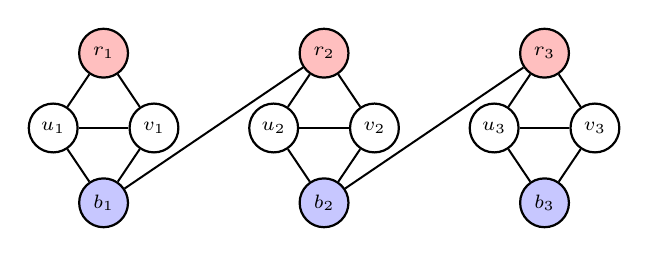
\begin{tikzpicture}[
   vertex/.style={circle,draw,thick,minimum size=6.2mm,inner sep=0pt,
      font=\scriptsize},
   redvertex/.style={vertex,fill=red!25},
   bluevertex/.style={vertex,fill=blue!22},
   whitevertex/.style={vertex,fill=white},
   edge/.style={line width=0.72pt}
]
   \foreach \i/\x in {1/0,2/2.8,3/5.6} {
      \node[redvertex] (r\i) at (\x,0.95) {\(r_{\i}\)};
      \node[bluevertex] (b\i) at (\x,-0.95) {\(b_{\i}\)};
      \node[whitevertex] (u\i) at ({\x-0.64},0) {\(u_{\i}\)};
      \node[whitevertex] (v\i) at ({\x+0.64},0) {\(v_{\i}\)};

      \draw[edge] (u\i) -- (v\i);
      \draw[edge] (r\i) -- (u\i);
      \draw[edge] (r\i) -- (v\i);
      \draw[edge] (b\i) -- (u\i);
      \draw[edge] (b\i) -- (v\i);
   }
   \draw[edge] (b1) -- (r2);
   \draw[edge] (b2) -- (r3);
\end{tikzpicture}
\caption{A connected graph $G$ with  \(\iso(G)=3\) and
\(\gamma_{\dsi}(G)=6\).}
\label{fig:diamond-chain-equality}
\end{figure}

We next give a lower bound on the dual-server independent domination number of a graph $G$ in terms of its diameter, denoted \(\diam(G)\).  Let \(d_G(u,v)\) denote the distance between vertices $u$ and $v$ in $G$.

This inequality was generated by \TheoConjecture{} as a conjecture.

\begin{theorem}
\label{thm:diameter}
If \(G\) is a nontrivial connected graph, then
\[
   \gamma_{\dsi}(G)\ge \left\lceil \frac{\diam(G)}{2}\right\rceil+1.
\]
Moreover, the bound is sharp for every possible value of the diameter.
\end{theorem}

\begin{proof}
Let \(d=\diam(G)\), and let
\[
   P=v_0v_1\cdots v_d
\]
be a diametral path in \(G\). Let \(S=R\cup B\) be a DSI-dominating set of
\(G\), and let \(k=|S|\) and \(t=|S\cap V(P)|\). We count the pairs
\((s,v_i)\), where \(s\in S\), \(0\le i\le d\), and \(s\in N[v_i]\).

For a fixed vertex \(s\in S\), there are at most three indices \(i\) for
which \(s\in N[v_i]\). Indeed, if \(s\in N[v_i]\cap N[v_j]\), then
\(d_G(v_i,v_j)\le 2\). Since \(P\) is a geodesic path, the subpath of \(P\)
from \(v_i\) to \(v_j\) is  a shortest $v_i$-$v_j$-path, and hence, \(|i-j|\le 2\). Thus, the
indices \(i\) with \(s\in N[v_i]\) are contained in three consecutive
positions. Therefore, the total number of counted pairs is at most \(3k\).

On the other hand, each vertex of \(S\cap V(P)\) contributes at least one
pair, namely the pair in which it counts itself. Each vertex of
\(V(P)\setminus S\) has a red neighbor and a blue neighbor in \(S\), and
these two neighbors are distinct. Hence, each vertex of \(V(P)\setminus S\)
contributes at least two pairs. It follows that
\[
   3k\ge t+2(d+1-t)=2d+2-t.
\]
Since \(t\le k\), we obtain
\[
   3k\ge 2d+2-k,
\]
and so \(4k\ge 2d+2\). Consequently, \(k\ge (d+1)/2\).

If \(d\) is even, then since \(k\) is an integer, this  gives
\[
   k\ge \left\lceil \frac d2\right\rceil+1.
\]
Assume now that \(d=2q+1\) is odd. The preceding inequality gives
\(k\ge q+1\). Suppose, for a contradiction, that \(k=q+1\). Then equality
holds throughout the preceding counting argument. In particular \(t=k\), so
every vertex of \(S\) lies on \(P\), and every selected vertex must be counted
by exactly three vertices of \(P\). Since all selected vertices lie on \(P\),
neither endpoint \(v_0\) nor \(v_d\) can lie outside \(S\), for otherwise, it would have at most one selected neighbor on \(P\) and no selected
neighbor outside \(P\). Thus, \(\{v_0,v_d\} \subseteq S\). But an endpoint of a geodesic
path is contained in the closed neighborhoods of at most two vertices of
\(P\), contradicting the requirement that every selected vertex be counted
exactly three times. Therefore, \(k\ge q+2\), which is precisely
\[
   k\ge \left\lceil \frac d2\right\rceil+1.
\]
Since \(S\) was arbitrary, the desired lower bound follows.

To see that the bound is sharp, take \(G=P_n\) with \(n\ge 2\). By
Proposition~\ref{prop:path-values},
\[
   \gamma_{\dsi}(P_n)=\left\lceil\frac{n+1}{2}\right\rceil.
\]
Since \(\diam(P_n)=n-1\), this is exactly
\[
   \left\lceil\frac{\diam(P_n)}{2}\right\rceil+1.
\]
Thus, equality holds for paths, and hence, for every positive value of the
diameter.
\end{proof}


We note that there is no forbidden subgraph characterization of graphs attaining the bound of  Theorem~\ref{thm:diameter}.  To show this, we construct a family  of extremal graphs admitting any arbitrary subgraph.  For $d \ge 2$, let $\cF_d$ be the family of graphs that can be obtained from a path \(P=v_0v_1\cdots v_d\)  with a given  $\gamma_{\dsi}$-set  $S= R \cup B$ and  associated 
DSI-partition. For each vertex \(v_i\notin S\), replace
\(v_i\) by an arbitrary nonempty graph \(H_i\), joining every vertex of
\(H_i\) to \(v_{i-1}\) and \(v_{i+1}\), and adding no other edges incident
with \(H_i\). Keep the selected vertices of \(P\) unchanged.   
For an example of a graph $G \in \cF_6$ , see  Figure~\ref{fig:diameter-blowup}, where  \(R = \{v_0,v_4\}\), \(B = \{v_2,v_6\}\), and \(S = R \cup B\).   The selected
vertices \(v_0,v_2,v_4,v_6\) retain the optimal red-blue coloring of the
path, while the unselected vertices \(v_1,v_3,v_5\) have been replaced by
nonempty white graphs \(H_1 = K_2, H_3 = \barK_2\), and \(H_5 = K_1\). Every white vertex sees both adjacent
colors, and the structure preserves the diameter of the path.

\begin{figure}[H]
\centering
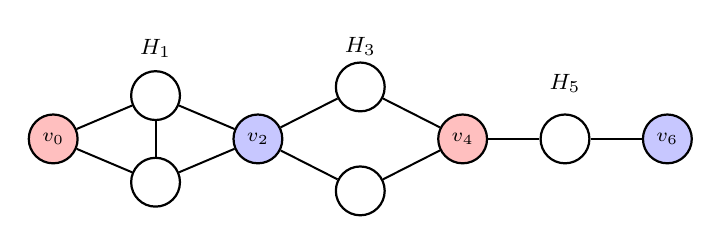
\begin{tikzpicture}[
   vertex/.style={circle,draw,thick,minimum size=6.2mm,inner sep=0pt,
      font=\scriptsize},
   redvertex/.style={vertex,fill=red!25},
   bluevertex/.style={vertex,fill=blue!22},
   whitevertex/.style={vertex,fill=white},
   edge/.style={line width=0.72pt}
]
   \node[redvertex] (v0) at (0,0) {\(v_0\)};
   \node[bluevertex] (v2) at (2.6,0) {\(v_2\)};
   \node[redvertex] (v4) at (5.2,0) {\(v_4\)};
   \node[bluevertex] (v6) at (7.8,0) {\(v_6\)};

   \node[whitevertex] (h11) at (1.3,0.55) {};
   \node[whitevertex] (h12) at (1.3,-0.55) {};
   \node[font=\footnotesize] at (1.3,1.15) {\(H_1\)};

   \node[whitevertex] (h31) at (3.9,0.66) {};
   \node[whitevertex] (h32) at (3.9,-0.66) {};
   \node[font=\footnotesize] at (3.9,1.18) {\(H_3\)};

   \node[whitevertex] (h51) at (6.5,0) {};
   \node[font=\footnotesize] at (6.5,0.70) {\(H_5\)};

   \draw[edge] (h11) -- (h12);
   %\draw[edge] (h31) -- (h32);

   \foreach \x in {h11,h12} {
      \draw[edge] (v0) -- (\x);
      \draw[edge] (v2) -- (\x);
   }
   \foreach \x in {h31,h32} {
      \draw[edge] (v2) -- (\x);
      \draw[edge] (v4) -- (\x);
   }
   \draw[edge] (v4) -- (h51);
   \draw[edge] (v6) -- (h51);
\end{tikzpicture}
\caption{A graph $G \in \cF_6$ with \(\gamma_{\dsi}(G) = 4\) and \(\diam(G) = d=6.\)}
\label{fig:diameter-blowup}
\end{figure}



\begin{proposition}
\label{prop:diameter-path-blowups}
If $G \in \cF_d$, then  
\[
   \diam(G)=d
   \quad\text{and}\quad
   \gamma_{\dsi}(G)=\left\lceil \frac d2\right\rceil+1.
\]
\end{proposition}
\begin{proof}  For $d \ge 2$, let \(G \in \cF_d\) be obtained from the  path \(P=v_0v_1\cdots v_d\)  with a given  $\gamma_{\dsi}$-set  $S= R \cup B$ and  associated 
DSI-partition.  By the construction of \(G\), we deduce that $S = R \cup B$ is a 
a DSI-dominating set of \(G\). Consequently,
\[
   \gamma_{\dsi}(G)\le |S|=\gamma_{\dsi}(P_{d+1})
      =\left\lceil\frac{d+2}{2}\right\rceil
      =\left\lceil\frac d2\right\rceil+1.
\]

It remains to check that \(\diam(G) = d = \diam(P)\).  By Observation~\ref{ob:leaf}, the vertices \(v_0\) and \(v_d\) are in  \(S\), and hence are not replaced  when forming  \(G\).  By the construction of \(G\), we deduce that \(d_G(v_0,v_d) = d_P(v_0,v_d) = d\), implying that \(\diam(G)\ge d\).

Conversely, we observe that $\diam(G) \le d$ as follows.  For a vertex $v_i \in V(P) \setminus S$, we let $u_i$ denote an arbitrary vertex in the replacement graph $H_i$.
For any $i, j, k \in [d]$, we deduce, from the construction of $G$, that \(d_G(v_i,u_j) = d_P(v_i,v_j)  \le d\) and  \(d_G(u_j,u_k) = d_P(v_j,v_k)  \le d\), where $v_i \in S$, $v_j, v_k \in V(P) \setminus S$, $u_j \in V(H_j)$, and $u_k \in V(H_k)$.  Moreover, the construction implies that $d_G(v_i,v_j) = d_P(v_i,v_j)  \le d$  for any  two vertices \(v_i\) and \(v_j\) in \(S\). Finally, for a vertex $v_i \in V(P) \setminus S$, any  two vertices in the replacement graph \(H_i\) are at
distance at most \(2 \le d\) in $G$, since both are adjacent to \(v_{i-1}\) and
\(v_{i+1}\).  
 
 Hence, \(\diam(G)\le d\), and so
\(\diam(G)=d\). The lower bound in Theorem~\ref{thm:diameter} now forces
equality for \(\gamma_{\dsi}(G)\).
\end{proof}

\begin{corollary}  There is no forbidden subgraph characterization of the graphs attaining the lower bound of Theorem~\ref{thm:diameter}.
\end{corollary}


 The
\emph{decycling number} \(\dec(G)\) is the minimum cardinality of a set
whose deletion leaves a forest, and the \emph{forest number}
\(\forest(G)\) is the maximum order of an induced forest in \(G\).

\begin{proposition}
\label{prop:decycling-forest}
For every graph \(G\) of order~$n$,
\[
   \forest(G)+\dec(G)=n.
\]
\end{proposition}

\begin{proof}
Let \(P\) be the property of being a forest. This property is hereditary in
the sense of Hedetniemi~\cite{Hedetniemi73}: every subgraph of a forest is a
forest. In the notation of~\cite{Hedetniemi73}, \(\beta_0(P)\) is the maximum
number of vertices in a set that induces a graph with property \(P\), and
\(\alpha_0(P)\) is the minimum number of vertices in a set meeting every
subgraph that does not have property \(P\). For \(P\) equal to being a
forest, these two quantities are precisely \(\forest(G)\) and \(\dec(G)\),
respectively: a vertex set meets every nonforest subgraph if and only if its
deletion leaves a forest. Hedetniemi's Theorem~\cite[Theorem~2]{Hedetniemi73}
gives \(\alpha_0(P)+\beta_0(P)=n\), and the result follows.
\end{proof}

The next proposition verifies, under the additional hypothesis that \(G\)
has an IDS-dominating set, the \TheoConjecture{} conjecture
\(\gamma_{\dsi}(G)\le n-\dec(G)\).

\begin{proposition}
\label{prop:ids-forest} If $G$ is a graph of order~$n$ and $G$ has an 
IDS-dominating set, then
\[
   \gamma_{\dsi}(G)\le i_{\ds}(G)\le \forest(G)=n-\dec(G).
\]
\end{proposition}

\begin{proof}
Let \(S\) be an \(i_{\ds}\)-set of \(G\). Since \(S\) is independent,
\(G[S]\) is an empty forest, and so \(|S|\le \forest(G)\). Thus,
\(i_{\ds}(G)\le \forest(G)\). The equality
\(\forest(G)=n-\dec(G)\) follows from
Proposition~\ref{prop:decycling-forest}, and
\(\gamma_{\dsi}(G)\le i_{\ds}(G)\) follows from
Observation~\ref{obs:basic-chain}.
\end{proof}

For DSI-domination, the corresponding hereditary
property is induced bipartiteness. Let \(\bipnum(G)\) be the
\emph{bipartite number} of \(G\), the maximum order of an induced bipartite
subgraph of \(G\), and let \(\bipcov(G)\) be the \emph{bipartite covering
number} of \(G\), the minimum cardinality of a set whose deletion leaves a
bipartite graph.

\begin{proposition}
\label{prop:bipartite-hereditary}
For every graph \(G\) of order~$n$,
\[
   \bipcov(G)+\bipnum(G)=n.
\]
\end{proposition}

\begin{proof}
This is the instance of Hedetniemi's Theorem~\cite[Theorem~2]{Hedetniemi73}
for the hereditary property of being bipartite.
\end{proof}

\begin{proposition}
\label{prop:dsi-bipartite-number}
For every nontrivial graph \(G\),
\[
   \gamma_{\dsi}(G)\le \bipnum(G).
\]
Furthermore,  if $G$ has an IDS-set, then
\[\gamma_{\dsi}(G) \le i_{\ds}(G) \le \alpha(G) \le \bipnum(G).\]
\end{proposition}

\begin{proof}
Let \(S\) be a \(\gamma_{\dsi}\)-set of \(G\), and let \(S=R\cup B\) be a
DSI-partition. Since \(R\) and \(B\) are independent, \(G[S]\) is bipartite
with bipartition \(\{R,B\}\). Hence, \(|S|\le \bipnum(G)\), and therefore, 
\(\gamma_{\dsi}(G)\le \bipnum(G)\).

If $G$ has an $i_{\ds}$-set $S$, then since $S$ is independent, $2 \le i_{\ds}(G) = |S| \le \alpha(G)$.   Every independent set of cardinality at least~2 induces a bipartite, so $\alpha(G) \le \bipnum(G)$.  
\end{proof}


\section{Computation and Complexity}
\label{sec:computation}

We next present both a concrete optimization model for computing the dual-server independent domination number and the corresponding hardness result. The optimization model is
also useful for reproducibility and for automated conjecturing. In the
\TheoConjecture{} experiments, the \AddDefinition{} tool was used to add
\(\gamma_{\dsi}\) to the First Principles workspace parameter database. In
this workflow, the user supplied the mathematical definition, and the system
drafted a user-defined optimization model that was checked on small
examples before being used in larger searches. Once saved, the invariant
could be evaluated on graph families and example databases in the same way
as the built-in parameters, so that conjecture searches could compare
\(\gamma_{\dsi}\) with domination, distance, independence,
hereditary-subgraph, and other structural quantities. The binary integer
programming model below is the mathematical form of the entry used for
these computations.

The manuscript source, scripts, CSV files, LP files, CBC logs, solution
files, fixed seeds, and metadata for the computational experiments are
available in the public artifact repository
\ArtifactRepo. Paths cited below are relative to the root of that
repository.

Let \(G\) be a nontrivial graph. For each vertex \(v\in V(G)\), introduce
binary variables \(r_v\) and \(b_v\), where \(r_v=1\) means that \(v\) is
selected in the red class and \(b_v=1\) means that \(v\) is selected in the
blue class. Consider the following binary integer program:
\[
\begin{array}{ll}
\text{minimize} &
   \displaystyle \sum_{v\in V(G)}(r_v+b_v) \\[1.2em]
\text{subject to} &
   \displaystyle \sum_{v\in V(G)} r_v \ge 1, \\[0.8em]
&
   \displaystyle \sum_{v\in V(G)} b_v \ge 1, \\[0.8em]
&
   r_v+b_v\le 1
      \qquad\text{for every } v\in V(G), \\[0.8em]
&
   r_u+r_v\le 1
      \qquad\text{for every } uv\in E(G), \\[0.8em]
&
   b_u+b_v\le 1
      \qquad\text{for every } uv\in E(G), \\[0.8em]
&
   \displaystyle r_v+b_v+\sum_{u\in N(v)} r_u\ge 1
      \qquad\text{for every } v\in V(G), \\[1.2em]
&
   \displaystyle r_v+b_v+\sum_{u\in N(v)} b_u\ge 1
      \qquad\text{for every } v\in V(G), \\[1.2em]
&
   r_v,b_v\in\{0,1\}
      \qquad\text{for every } v\in V(G).
\end{array}
\tag{IP}
\]

The last two constraint families are the two-color domination constraints.
They say that each vertex \(v\) is either selected, meaning \(r_v+b_v=1\),
or has a red neighbor; and, independently, that \(v\) is either selected or
has a blue neighbor. Thus, if \(v\notin R\cup B\), then \(r_v=b_v=0\), and
both a red neighbor and a blue neighbor are required. If \(v\in R\cup B\),
then no domination requirement is imposed on \(v\) itself.


\begin{proposition}
\label{prop:ip-formulation}
For every nontrivial graph \(G\), the optimum value of \((\mathrm{IP})\) is
\(\gamma_{\dsi}(G)\).
\end{proposition}

\begin{proof}
Given a feasible solution of \((\mathrm{IP})\), let
\[
   R=\{v\in V(G): r_v=1\}
   \qquad\text{and}\qquad
   B=\{v\in V(G): b_v=1\}.
\]
The first two constraints require \(R\) and \(B\) to be nonempty, and the
third requires them to be disjoint. The edge constraints
\(r_u+r_v\le 1\) and \(b_u+b_v\le 1\) require \(R\) and \(B\) to be
independent. Finally, if \(v\notin R\cup B\), then \(r_v=b_v=0\), and the
two neighborhood constraints require \(v\) to have a neighbor in \(R\) and a
neighbor in \(B\). Thus, \(R\cup B\), with partition \(\{R,B\}\), is a
DSI-dominating set, and its cardinality is the value of the objective
function.

Conversely, if \(S=R\cup B\) is a DSI-dominating set with associated
DSI-partition, set \(r_v=1\) for \(v\in R\), set \(b_v=1\) for \(v\in B\),
and set all other variables equal to \(0\). The DSI conditions give every
constraint of \((\mathrm{IP})\), and the objective value is \(|S|\).
Therefore, the minimum possible objective value is exactly
\(\gamma_{\dsi}(G)\).
\end{proof}


We now turn to the decision version and show that, despite this compact
model, computing \(\gamma_{\dsi}(G)\) is computationally NP-complete.  Recall that a bipartite graph is \emph{chordal bipartite} if
every cycle of length at least six has a chord. The relevant decision problem
is the following.

\noindent\textsc{DSI-Domination}.

\textbf{Instance:} A nontrivial graph \(G\) of order~$n$ and a positive integer \(k\le
n\).

\textbf{Question:} Does \(G\) have a DSI-dominating set of cardinality at
most \(k\)?

\begin{theorem}
\label{thm:dsi-np-complete}
\textnormal{\textsc{DSI-Domination}} is NP-complete, even when restricted to
chordal bipartite graphs.
\end{theorem}

\begin{proof}
The problem belongs to \(\mathcal{NP}\), since a certificate consists of two
sets \(R,B\subseteq V(G)\). In polynomial time one verifies that \(R\) and
\(B\) are nonempty and disjoint, that both \(R\) and \(B\) are independent,
that \(|R\cup B|\le k\), and that every vertex outside \(R\cup B\) has a
neighbor in each of \(R\) and \(B\).

For hardness, we reduce from \textsc{Dominating Set} restricted to chordal
bipartite graphs, which is NP-complete by a theorem of M\"uller and
Brandst\"adt~\cite{MullerBrandstadt87}. Let \(H\) be a chordal bipartite
graph, let \(k\) be a positive integer with \(k\le |V(H)|\), and write
\(n=|V(H)|\). Construct a graph \(G\) from \(H\) by adding, for each
\(v\in V(H)\), a new leaf \(x_v\) adjacent only to \(v\). Let
\[
   L=\{x_v: v\in V(H)\}
   \qquad\text{and}\qquad
   K=n+k.
\]
The construction is polynomial. Since adding leaves creates no new cycles,
\(G\) is chordal bipartite whenever \(H\) is chordal bipartite.

Suppose first that \(H\) has a dominating set \(D\) with \(|D|\le k\). Fix a
bipartition \((A,B)\) of \(H\). We claim that \(S=L\cup D\) is a
DSI-dominating set of \(G\). Color the vertices of \(D\cap A\) red and the
vertices of \(D\cap B\) blue. For each \(v\in D\), color \(x_v\) opposite to
the color of \(v\). For each \(v\notin D\), color \(x_v\) red if \(v\in A\)
and blue if \(v\in B\). This is a proper red-blue coloring of \(G[S]\), so
both color classes are independent. Now let \(v\in V(H)\setminus D\). The
leaf \(x_v\) has the color corresponding to the part of \(H\) containing
\(v\), and since \(D\) dominates \(H\), the vertex \(v\) has a neighbor
\(u\in D\) in the other part, whose color is opposite to the color of
\(x_v\). Thus, every vertex outside \(S\) sees both colors, and
\(|S|=n+|D|\le K\).

Conversely, suppose that \(G\) has a DSI-dominating set \(S=R\cup B\) with
\(|S|\le K\). Every leaf \(x_v\) belongs to \(S\), for otherwise \(x_v\)
would have at most one selected neighbor and could not see both colors. Let
\(D=S\cap V(H)\). Since \(L\subseteq S\), we have
\[
   |D|\le |S|-|L|\le K-n=k.
\]
If \(v\in V(H)\setminus D\), then \(v\notin S\). Its selected neighbors in
\(G\) consist of \(x_v\) and the vertices in \(D\cap N_H(v)\). Since \(v\)
must see both color classes, it follows that \(D\cap N_H(v)\neq\emptyset\).
Thus, \(D\) is a dominating set of \(H\) of cardinality at most \(k\). This
proves the equivalence of the two decision instances.
\end{proof}

\begin{proposition}
\label{prop:bounded-treewidth}
For every fixed integer \(t\ge 0\), the value \(\gamma_{\dsi}(G)\) can be
computed in linear time on the class of nontrivial graphs satisfying treewidth 
\(\tw(G)\le t\). Consequently, \textnormal{\textsc{DSI-Domination}} is
polynomial-time solvable on every graph class of bounded treewidth.
\end{proposition}

\begin{proof}
We use the standard monadic second-order optimization framework for graphs of
bounded treewidth \cite{Courcelle90,CourcelleMakowskyRotics00}. Let
\(x\sim y\) denote adjacency. For vertex-set variables \(R\) and \(B\), consider
the following monadic second-order formula:
\[
\begin{aligned}
\Phi(R,B)\equiv{}&
   (\exists r\, r\in R)\land(\exists b\, b\in B)                                      \\
&{}\land \forall x\, \neg(x\in R\land x\in B)                                         \\
&{}\land \forall x\forall y\,
   \bigl((x\in R\land y\in R\land x\sim y)\rightarrow x=y\bigr)                       \\
&{}\land \forall x\forall y\,
   \bigl((x\in B\land y\in B\land x\sim y)\rightarrow x=y\bigr)                       \\
&{}\land \forall x\,
   \bigl((x\notin R\land x\notin B)\rightarrow
      (\exists y\,(y\in R\land x\sim y)\land
       \exists z\,(z\in B\land x\sim z))\bigr).
\end{aligned}
\]
The first line requires both color classes to be nonempty, the second requires
them to be disjoint, the next two require each color class to be independent,
and the final line requires every unselected vertex to have a neighbor in each
color class. Hence, a pair \((R,B)\) satisfies \(\Phi\) precisely when
\(R\cup B\), with its prescribed partition, is a DSI-dominating set.
Therefore,
\[
   \gamma_{\dsi}(G)=
   \min\{|R|+|B|:\, G\models \Phi(R,B)\}.
\]
Since \(\Phi\) is fixed, the Monadic Second-Order Optimization Theorem gives a
linear-time algorithm, for each fixed \(t\), to compute this minimum from a
tree-decomposition of width at most \(t\). Bodlaender's algorithm finds such a
tree-decomposition in linear time for fixed \(t\), or correctly reports that
the treewidth exceeds \(t\) \cite{Bodlaender96}. Combining these two algorithms
proves the claim.
\end{proof}



\section{\TheoConjecture{} Open Problems}

We conclude this paper with a sampling of the conjectures generated by
\TheoConjecture{} after the parameter \(\gamma_{\dsi}\) was added to the
First Principles automated conjecturing system. The conjectures below
resisted both human counterexample searches and counterexample attempts made
through the \CoPilot{} chat interface with the system. They represent
our favorite surviving conjectures from this process; several other
system-generated conjectures were found to be false, either by the authors
or by the AI system itself.

We use \(\avgdist(G)\) for the \emph{average distance} of a connected graph
\(G\). The \emph{domination
core} of \(G\), denoted
\(\Core(G)\), is the set of vertices that belong to every \(\gamma\)-set of
\(G\). A \emph{paired dominating set} of \(G\) is a dominating set \(D\) such
that \(G[D]\) contains a perfect matching; its minimum cardinality is the
\emph{paired domination number} \(\gamma_{\pr}(G)\)~\cite{HaynesSlater98}.
The conjectures are ordered as follows: first a mixed degree and paired
domination inequality, then two inequalities of the form
\(\gamma_{\dsi}(G)+\cdots\le n\), followed by two lower bounds, two upper
bounds, and finally an equality conjecture.

\begin{conjecture}[\TheoConjecture]
\label{conj:paired-degree}
If \(G\) is a nontrivial connected graph, then
\[
   \delta(G)\gamma_{\pr}(G)\le \Delta(G)\gamma_{\dsi}(G).
\]
\end{conjecture}

\begin{conjecture}[\TheoConjecture]
\label{conj:decycling-upper}
If \(G\) is a nontrivial graph of order~\(n\), then
\[
   \gamma_{\dsi}(G)+\dec(G)\le n.
\]
\end{conjecture}

\begin{conjecture}[\TheoConjecture]
\label{conj:core}
If \(G\) is a nontrivial connected graph, then
\[
   \gamma_{\dsi}(G)+|\Core(G)|\le n.
\]
\end{conjecture}

\begin{conjecture}[\TheoConjecture]
\label{conj:clawfree-average-distance}
If \(G\) is a nontrivial connected  claw-free graph, then
\[
   \gamma_{\dsi}(G)\ge
   \left\lceil \frac{3\avgdist(G)}{2}\right\rceil.
\]
\end{conjecture}

\begin{conjecture}[\TheoConjecture]
\label{conj:trianglefree-lower}
If \(G\) is a nontrivial connected triangle-free graph, then
\[
   \gamma_{\dsi}(G)\ge \dec(G)+1.
\]
\end{conjecture}

\begin{conjecture}[\TheoConjecture]
\label{conj:bipartite-number}
If \(G\) is a nontrivial connected  claw-free graph, then
\[
   \gamma_{\dsi}(G)\le \left\lfloor \frac{3\bipnum(G)}{4}\right\rfloor+1.
\]
\end{conjecture}

\begin{conjecture}[\TheoConjecture]
\label{conj:cubic-domination}
If \(G\) is a nontrivial connected cubic graph, then
\[
   \gamma_{\dsi}(G)\le 2\gamma(G).
\]
\end{conjecture}

\begin{conjecture}[\TheoConjecture]
\label{conj:bipartite-cubic}
If \(G\) is a nontrivial connected bipartite cubic graph, then
\[
   \gamma_{\dsi}(G)=\gamma_{\ds}(G).
\]
\end{conjecture}



\appendix

\section{Baseline Ensemble Illustrations}
\label{app:ensemble-experiment}

This appendix records two small baseline studies connected with the
ensemble-learning interpretation mentioned in the introduction. They are
included for reproducibility and motivation only. The purpose is not to
propose a new ensemble-learning algorithm, nor to claim that
DSI-domination is a competitive classifier-selection method. Instead, the
studies illustrate how the DSI constraint can be implemented as an exact
graph-theoretic diversity-and-coverage rule on a learner-dependence graph.
The first study uses synthetic data with known latent dependence families.
The second uses standard classification datasets and adds a simple
accuracy-aware refinement after the minimum DSI cardinality has been fixed.

\subsection{Synthetic Baseline}

In each trial, we generated \(48\) binary base predictors arranged in six
latent dependence families of eight predictors each. For each observation,
all predictors in the same family were affected by a shared error source,
and each predictor was also affected by an independent error source. The
learner graph was constructed from validation data by joining two predictors
when the phi-correlation of their validation error indicators was at least
\(0.15\). Thus, adjacency represents a strong tendency to err together. We
then solved the binary integer program \((\mathrm{IP})\) for a
DSI-dominating set, used the selected predictors in a majority vote on an
independent test set, and compared this vote with \(200\) uniformly random
same-size subsets of predictors. The baseline used \(30\) fixed random
seeds, \(1000\) validation observations, and \(3000\) test observations per
trial.

The raw data, fixed seeds, LP files, CBC logs, solution files, and metadata
are available in the artifact repository at
\path{computational_data/ensemble/}. The script
\path{computational_data/ensemble_dsi_experiment.py} regenerates the
baseline using only the Python standard library and the command-line CBC
solver.

\begin{table}[H]
\centering
\small
\begin{tabular}{lr}
\hline
Quantity & Value \\
\hline
Trials & 30 \\
Base predictors & 48 \\
Latent dependence families & 6 \\
Random same-size ensembles per trial & 200 \\
Trials solved optimally by CBC & 30 \\
Mean \(\gamma_{\dsi}\) of learner graph & 12.000 \\
Mean DSI majority-vote accuracy & 0.953911 \\
Mean random same-size majority-vote accuracy & 0.933030 \\
Mean accuracy difference & 0.020881 \\
Trials where DSI exceeded the random mean & 30 \\
Mean DSI accuracy percentile among random subsets & 0.951667 \\
Mean DSI average error correlation & 0.047216 \\
Mean random average error correlation & 0.078203 \\
Mean correlation difference & \(-0.030986\) \\
\hline
\end{tabular}
\caption{Aggregate results for the synthetic ensemble baseline. The random
accuracy and random error-correlation values are trialwise averages over
\(200\) random same-size subsets.}
\label{tab:ensemble-experiment}
\end{table}

In this synthetic model, the validation threshold recovered the latent
dependence families, and a minimum DSI-dominating set selected two
representatives from each family, one in each color class. The DSI selection
therefore had lower average pairwise error correlation than a random
same-size selection, while preserving coverage of the learner pool through
the domination condition. This is the only point of the synthetic baseline:
it verifies, in a controlled setting, that the graph-theoretic rule behaves
as the definition suggests.

\subsection{Standard-Data Baseline}

The second baseline uses four standard classification
datasets: Iris \cite{FisherUCI}, Palmer Penguins
\cite{HorstHillGorman20}, Wine \cite{AeberhardForinaUCI}, and Wisconsin
Diagnostic Breast Cancer \cite{WolbergMangasarianStreetUCI}. In each trial,
the data were split in a stratified \(60/20/20\) train-validation-test
proportion. We trained \(48\) simple base learners using only the Python
standard library: nearest-centroid classifiers, Gaussian naive Bayes
classifiers, \(k\)-nearest-neighbor classifiers, and decision stumps, with
both full and random feature subsets. Since diversity is useful only among
competent predictors, we first retained the learners whose validation
accuracy was within \(0.05\) of the best validation accuracy, keeping at
least \(16\) candidates. The learner graph was then formed on this candidate
pool by joining the top \(25\%\) of pairs by validation-set prediction
agreement. A minimum DSI-dominating set was computed by the binary integer
program from Section~\ref{sec:computation}, and its majority vote was
evaluated on the test set. We also computed an accuracy-aware
lexicographic refinement. Namely, after first determining
\(\gamma_{\dsi}\) for the learner graph, we maximized, among DSI-dominating
sets of this minimum cardinality, the number of validation examples on
which the correct class received a strict plurality vote from the selected
learners. Individual validation accuracy was used only as a small
tie-breaker. We call this second-stage rule VM-DSI. It preserves the exact
DSI size constraint while letting the
second-stage optimization distinguish between minimum DSI sets that are
equally good from the graph-theoretic point of view.

The raw data files, fixed seeds, trial-level CSV file, summary CSV file, LP
files, CBC logs, solution files, and metadata are available in the artifact
repository at \path{computational_data/real_data/}. The script
\path{computational_data/real_data_dsi_experiment.py} regenerates the
baseline using only the Python standard library and the command-line CBC
solver.

\begin{table}[H]
\centering
\scriptsize
\begin{tabular}{lrrrrrrrrr}
\hline
Dataset & Cand. & \(\gamma_{\dsi}\) & DSI acc. & VM-DSI acc. &
Top-\(k\) acc. & Rand. acc. & Full acc. & VM agr. & Rand. agr. \\
\hline
Iris & 17.950 & 6.650 & 0.940 & 0.947 & 0.950 & 0.944 & 0.945 & 0.946 & 0.951 \\
Penguins & 16.000 & 8.800 & 0.964 & 0.965 & 0.992 & 0.985 & 0.989 & 0.808 & 0.862 \\
WDBC & 16.150 & 7.800 & 0.954 & 0.958 & 0.964 & 0.957 & 0.961 & 0.919 & 0.928 \\
Wine & 16.000 & 6.800 & 0.969 & 0.963 & 0.961 & 0.966 & 0.971 & 0.883 & 0.901 \\
\hline
\end{tabular}
\caption{Aggregate results for the standard-data ensemble baseline.
Each row reports \(20\) stratified train-validation-test splits. ``Cand.''
is the mean number of validation-competent candidate learners. VM-DSI is
the validation-margin DSI refinement. The random accuracy and random
agreement values are trialwise averages over \(200\) random same-size
subsets of the candidate pool. Agreement is the mean pairwise test-set
prediction agreement within the selected ensemble.}
\label{tab:real-data-ensemble-experiment}
\end{table}

These data should be read cautiously. The minimum DSI rule is an exact
graph-theoretic selection rule, not an accuracy-aware ensemble objective.
The validation-margin refinement is more faithful to the ensemble-learning
interpretation: it keeps the same DSI cardinality but uses validation data
to choose among the minimum DSI sets. Even then, the goal is illustrative
rather than competitive. On these small datasets, VM-DSI keeps test
accuracy near the natural baselines while retaining lower pairwise
agreement than random same-size selections. Thus, the standard-data baseline
supports a modest interpretation: DSI-domination can serve as a
mathematically clean diversity-and-coverage primitive inside a larger
ensemble-selection pipeline, but further accuracy-aware variants would be
needed before presenting it as a standalone machine learning method.

\begin{thebibliography}{99}

\bibitem{AeberhardForinaUCI}
S. Aeberhard and M. Forina,
Wine [Dataset],
UCI Machine Learning Repository, 1992,
doi:10.24432/C5PC7J.

\bibitem{Allan78}
R. B. Allan and R. Laskar,
On domination and independent domination numbers of a graph,
\emph{Discrete Math.} \textbf{23} (1978), 73--76.

\bibitem{Blidia06}
M. Blidia, M. Chellali, and O. Favaron,
Ratios of some domination parameters in graphs and claw-free graphs,
in \emph{Graph Theory}, Trends in Mathematics, Birkh\"auser, Basel, 2006,
61--72.

\bibitem{Blidia05}
M. Blidia, M. Chellali, and O. Favaron,
Independence and 2-domination in trees,
\emph{Australas. J. Combin.} \textbf{33} (2005), 317--327.

\bibitem{BlidiaChellaliVolkmann06}
M. Blidia, M. Chellali, and L. Volkmann,
Bounds of the 2-domination number of graphs,
\emph{Utilitas Math.} \textbf{71} (2006), 209--216.

\bibitem{Bodlaender96}
H. L. Bodlaender,
A linear-time algorithm for finding tree-decompositions of small treewidth,
\emph{SIAM J. Comput.} \textbf{25} (1996), 1305--1317.

\bibitem{chh}
M. Chellali, T. W. Haynes, and S. T. Hedetniemi,
Dual-server domination in graphs,
\emph{Discrete Appl. Math.} \textbf{387} (2026), 251--259.

\bibitem{Brown05}
G. Brown, J. Wyatt, R. Harris, and X. Yao,
Diversity creation methods: a survey and categorisation,
\emph{Information Fusion} \textbf{6} (2005), 5--20.

\bibitem{CaroHansberg17}
Y. Caro and A. Hansberg,
Partial domination -- the isolation number of a graph,
\emph{Filomat} \textbf{31} (2017), 3925--3944.

\bibitem{Courcelle90}
B. Courcelle,
The monadic second-order logic of graphs. I. Recognizable sets of finite
graphs,
\emph{Inform. and Comput.} \textbf{85} (1990), 12--75.

\bibitem{CourcelleMakowskyRotics00}
B. Courcelle, J. A. Makowsky, and U. Rotics,
Linear time solvable optimization problems on graphs of bounded clique-width,
\emph{Theory Comput. Syst.} \textbf{33} (2000), 125--150.

\bibitem{DavilaTxGraffiti}
R. Davila,
Automated conjecturing with TxGraffiti,
\emph{Ann. Math. Artif. Intell.} (2026), doi:10.1007/s10472-026-10005-5.

\bibitem{DavilaGraffiti3}
R. Davila,
Graffiti3: Compact theory libraries for automated mathematical discovery,
Research Square preprint, 2026, doi:10.21203/rs.3.rs-8493329/v1.

\bibitem{Dietterich00}
T. G. Dietterich,
Ensemble methods in machine learning,
in \emph{Multiple Classifier Systems},
Lecture Notes in Computer Science \textbf{1857}, Springer, Berlin, 2000,
1--15.

\bibitem{DafoeEtAl20}
A. Dafoe, E. Hughes, Y. Bachrach, T. Collins, K. R. McKee, J. Z. Leibo,
K. Larson, and T. Graepel,
Open problems in cooperative AI,
arXiv:2012.08630, 2020.

\bibitem{DelavinaLarsonPepperWaller10}
E. DeLaVi\~na, C. E. Larson, R. Pepper, and B. Waller,
Graffiti.pc on the 2-domination number of a graph,
\emph{Congr. Numer.} \textbf{203} (2010), 15--32.

\bibitem{FisherUCI}
R. A. Fisher,
Iris [Dataset],
UCI Machine Learning Repository, 1936,
doi:10.24432/C56C76.

\bibitem{Fink85}
J. F. Fink and M. S. Jacobson,
\(n\)-domination in graphs,
in \emph{Graph Theory with Applications to Algorithms and Computer Science},
Wiley, New York, 1985, 283--300.

\bibitem{Harary00}
F. Harary and T. W. Haynes,
Double domination in graphs,
\emph{Ars Combin.} \textbf{55} (2000), 201--213.

\bibitem{HaynesSlater98}
T. W. Haynes and P. J. Slater,
Paired-domination in graphs,
\emph{Networks} \textbf{32} (1998), 199--206.

\bibitem{GoddardHenning25}
W. Goddard and M. A. Henning,
On the isolation number of graphs with minimum degree four,
arXiv:2508.21551, 2025.

\bibitem{hhh1}
T. W. Haynes, S. T. Hedetniemi, and M. A. Henning (eds.),
\emph{Topics in Domination in Graphs},
Developments in Mathematics \textbf{64}, Springer, Cham, 2020.

\bibitem{hhh2}
T. W. Haynes, S. T. Hedetniemi, and M. A. Henning (eds.),
\emph{Structures of Domination in Graphs},
Developments in Mathematics \textbf{66}, Springer, Cham, 2021.

\bibitem{hhh3}
T. W. Haynes, S. T. Hedetniemi, and M. A. Henning,
\emph{Domination in Graphs: Core Concepts},
Springer Monographs in Mathematics, Springer, Cham, 2023.

\bibitem{HHHS}
T. W. Haynes, S. T. Hedetniemi, M. A. Henning, and P. J. Slater,
\(H\)-forming sets in graphs,
\emph{Discrete Math.} \textbf{262} (2003), 159--169.

\bibitem{HorstHillGorman20}
A. M. Horst, A. P. Hill, and K. B. Gorman,
\emph{palmerpenguins: Palmer Archipelago (Antarctica) Penguin Data},
R package version 0.1.0, 2020,
doi:10.5281/zenodo.3960218.

\bibitem{Hedetniemi08}
S. M. Hedetniemi, S. T. Hedetniemi, R. C. Laskar, L. Markus, and P. J. Slater,
Disjoint dominating sets in graphs,
\emph{Proc. Internat. Conf. Discrete Math., ICDM 2006},
Ramanujan Math. Soc. Lect. Notes Ser. \textbf{7} (2008), 87--100.

\bibitem{Hedetniemi73}
S. T. Hedetniemi,
Hereditary properties of graphs,
\emph{J. Combin. Theory Ser. B} \textbf{14} (1973), 94--99.

\bibitem{IrvingChristianoAmodei18}
G. Irving, P. Christiano, and D. Amodei,
AI safety via debate,
arXiv:1805.00899, 2018.

\bibitem{Kuncheva04}
L. I. Kuncheva,
\emph{Combining Pattern Classifiers: Methods and Algorithms},
John Wiley \& Sons, Hoboken, NJ, 2004.

\bibitem{LiuYao99}
Y. Liu and X. Yao,
Ensemble learning via negative correlation,
\emph{Neural Networks} \textbf{12} (1999), 1399--1404.

\bibitem{MullerBrandstadt87}
H. M\"uller and A. Brandst\"adt,
The NP-completeness of Steiner tree and dominating set for chordal bipartite
graphs,
\emph{Theoret. Comput. Sci.} \textbf{53} (1987), 257--265.

\bibitem{Peters86}
K. W. Peters,
\emph{Theoretical and Algorithmic Results on Domination and Connectivity},
Ph.D. thesis, Clemson University, 1986.

\bibitem{ShohamLeytonBrown08}
Y. Shoham and K. Leyton-Brown,
\emph{Multiagent Systems: Algorithmic, Game-Theoretic, and Logical
Foundations},
Cambridge University Press, Cambridge, 2008.

\bibitem{Sumner90}
D. P. Sumner,
Critical concepts in domination,
\emph{Discrete Math.} \textbf{86} (1990), 33--46.

\bibitem{Wooldridge09}
M. Wooldridge,
\emph{An Introduction to MultiAgent Systems},
2nd ed., John Wiley \& Sons, Chichester, 2009.

\bibitem{WolbergMangasarianStreetUCI}
W. Wolberg, O. Mangasarian, N. Street, and W. Street,
Breast Cancer Wisconsin (Diagnostic) [Dataset],
UCI Machine Learning Repository, 1993,
doi:10.24432/C5DW2B.

\end{thebibliography}

\end{document}
